%20/10 - Kostadin
\chapter{Introducción al lenguaje}
\section{Textos}

Los humanos nos comunicamos principalmente de forma oral, y el texto es la representación escrita de ese habla. Los animales también se comunican, usualmente sobre el estado actual o presente. El texto es una abreviación del habla, una forma de transcribirla con ciertas características:
\begin{itemize}
\item Es muy comprimido: el habla se produce mediante la acción de los músculos controlados por la corteza motora. Estamos limitados a emitir una cadena unidimensional de sonidos o fonemas.
\item Las categorías de sonido están acotadas y corresponden a los morfemas del lenguaje. Al escribir los morfemas, ya tenemos el texto.
\item El texto se transmite a través de letras, símbolos discretos.
\end{itemize}

El texto es una transcripción de una señal sonora que mantiene sus propiedades esenciales. Puede copiarse indefinidamente y es resistente al ruido.

El objetivo de la minería de textos es extraer información relevante de textos escritos. Algunos términos clave son:
\begin{itemize}
\item Información: Una letra es una unidad de información. Un dígito tiene menos opciones (0-9) comparado con las letras (a-z), por lo que posee menos información. Para codificar todo el abecedario se requieren al menos dos dígitos. La cantidad de información depende del número de posibles mensajes. Por ejemplo, con un dígito hay 10 posibilidades, con dos dígitos 100, y con tres dígitos 1000. En informática, se usan dos dígitos binarios (0 y 1). El logaritmo en base 2 mide la información en bits: 
$log_2(3) \approx 10$.
\item Relevancia: Algo es relevante si está relacionado con un problema específico. Por ejemplo, si buscamos una sustancia que cause diabetes en ratones, lo relevante es todo lo que se relacione con esa sustancia. La relevancia depende del problema concreto.
\item Fiabilidad: Debemos trabajar con información fiable, preferiblemente basada en la realidad y datos experimentales.
\item Texto humano: Tiene una estructura que viene de la secuencia continua de movimientos musculares al hablar. Además, existe una estructura jerárquica dada por la gramática y la sintaxis.
\end{itemize}

La redundancia garantiza robustez ante el ruido. El texto es redundante en varios niveles:
\begin{enumerate}
\item Fonemas: un fonema, como la vocal "a", tiene una duración corta (décimas de segundo). Si parte de la señal se pierde, otras repeticiones ayudan a comprenderlo.
\item Variaciones pequeñas en sonidos o escritura normalmente no afectan al significado. Por ejemplo, quitando las vocales, aún podemos entender un texto. Muchos lenguajes antiguos, como el árabe o los lenguajes semitas, no escriben vocales. Estas se introdujeron para facilitar la lectura sin conocer el contexto.
 \end{enumerate}

Ejercicio: estimar la velocidad de transmisión entre humanos de texto en dos contextos: uno escribe y el otro lo recibe; uno lee algo ya escrito como una novela. No se puede estimar la información, solo un límite superior a la información ("no más que x"). %Esto no hay quien lo entienda
\begin{itemize}
 \item Vídeo: 5 000 000 bits por segundo
 \item Teléfono: 3 000 bps
 \item Radio: 20 000 bps
 \item Leer (para uno mismo, en silencio): de media 200 palabras por minuto, unas 1000 letras por minuto. Siendo 6 bits la letra, 6000 bits por minuto o 100 bps.
 \item Escribir un texto: 60-90 palabras por minuto, con una media de 5 letras por palabra: 360-540 letras por minuto. Siendo 6 bits la letra, sale 40-60 bps
\end{itemize}

No toda comunicación es habla humana. Por ejemplo, si una persona describe algo para que otra lo dibuje, la información transmitida será muy diferente.
Tenemos diferentes tipos de señales: sonora o de letras. En términos de información, la función $f(x)$ tiene menos información que su argumento $x$, es decir, $f(x) < x$. 

\section{Artículos}
La mayoría de la información científica se encuentra en artículos. Un artículo es un texto publicado que puede incluir imágenes y fórmulas. Los artículos científicos y periodísticos se parecen: ambos tienen autores y reflejan la opinión de éstos. El artículo es una función de la información del evento, por lo que contiene menos información que el propio evento. Los autores están limitados por sus conocimientos y la fuente de información a la que acceden, como vídeos, relatos, testimonios, etc. El tiempo de escritura es también importante; el autor produce la mejor versión posible en ese momento, dentro de su contexto.

Un artículo de una página de periódico suele tener unas 300 palabras. Este valor puede obtenerse comprimiendo el contexto y el artículo.

En artículos científicos existe cierto grado de censura; no todo lo que sabe el autor se incluye. Cuanto más accesible es el artículo, mejor, por eso existen iniciativas OpenSource. Existen varios tipos de artículos científicos: investigación original, reviews (revisión de varios trabajos), propuestas metodológicas, estudios de caso (case studies, con potencia estadística limitada) y opiniones.

Un artículo cercano a la realidad contiene más información. Las fuentes más fieles incluyen historiales clínicos, diarios de laboratorio, datos estadísticos, comunicaciones entre personas sobre hechos, y datos del Internet of Things.

Actualmente, también están disponibles fuentes preprocesadas por inteligencia artificial (IA), que son modelos estadísticos del lenguaje. Reflejan la opinión prevalente, pero no su diversidad, tienen un horizonte temporal limitado, y un retraso por el tiempo de entrenamiento. Estas fuentes pueden reforzar opiniones dominantes debido a feedback positivo. Por ello, es recomendable complementar búsquedas IA con consultas directas a la web, aunque gran parte de la información en la web también ha pasado por IA.

\section{Minería de datos}
La minería de textos analiza uno o varios textos para responder preguntas como: ¿de qué trata? ¿Es fiable? ¿Tiene interés? ¿Qué información contiene y cómo describirla? ¿Cuál es la información nueva? ¿Cómo presentar la información de forma estructurada?
Los formatos estructurados incluyen bases de datos relacionales, no relacionales, grafos y programas.

Ejercicio: Food Insecurity Interventions to Improve Blood Pressure - JAMA Internal Medicine. 
El artículo tiene información no textual, está en los gráficos. Tiene 458 participantes, que está bien en cuanto a potencia estadística. 

Los \textbf{datos estructurados} tienen organización clara, fáciles de consultar, modificar y analizar, y suelen ser isomórficos con tablas relacionadas. Ejemplos: bases de datos, hojas Excel, gráficos conceptuales, datos de formularios.

Los \textbf{datos no estructurados} carecen de un modelo fijo, están en formatos naturales mezclando información útil con redundante, y no se pueden organizar trivialmente en tablas. Ejemplos: texto, vídeo, imagen.

El hipertexto es texto con relaciones internas o externas. Se estima que el 80\% de los datos son no estructurados.

\begin{figure}[h]
\centering
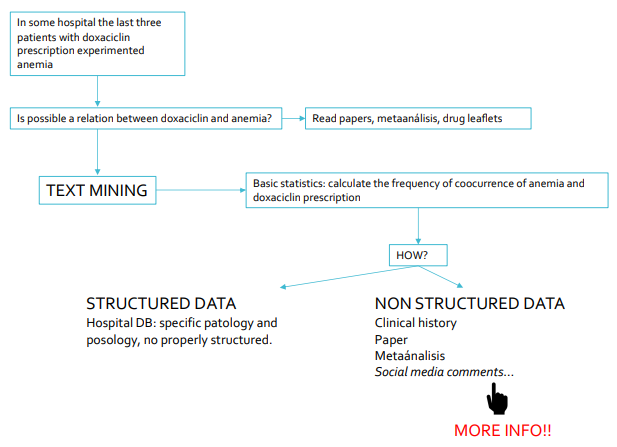
\includegraphics[width = \textwidth]{figs/ej-mineria.png}
\end{figure}

El trabajo fundamental en procesamiento de lenguaje natural es transformar datos no estructurados en estructurados. La idoneidad del método depende de la tarea real.
Dos grandes grupos de métodos:
\begin{itemize}
\item Métodos clásicos: dividir una tarea compleja en subtareas simples (p. ej. sistema de preguntas y respuestas basado en etiquetado POS, análisis sintáctico, reconocimiento de entidades nombradas) y combinarlas para generar la respuesta en lenguaje natural.
\item Métodos basados en aprendizaje profundo: un sistema único que procesa grandes cantidades de texto para crear una representación interna útil a la tarea.
\end{itemize}

\begin{figure}[h]
\centering
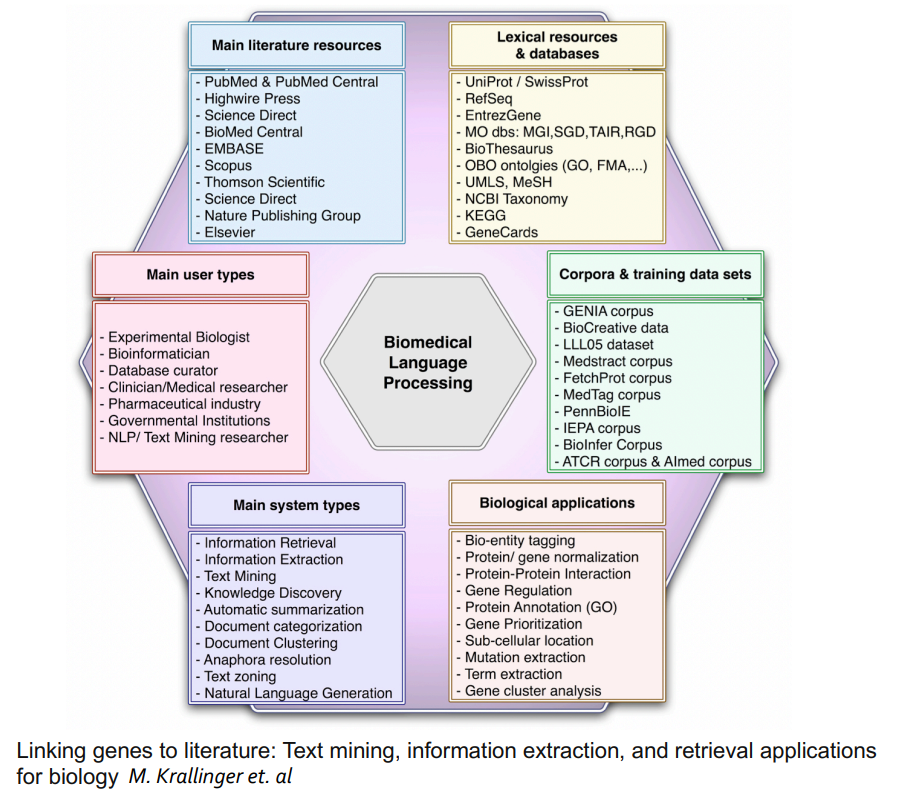
\includegraphics[width = 0.6\textwidth]{figs/blp.png}
\end{figure}

La pipeline del NLP funciona de la siguiente forma:
\begin{enumerate}
\item Extracción de datos de texto: Selección de las fuentes de datos de texto, aplicación de diferentes técnicas de consulta, API REST, extracción de datos web, consulta de bases de datos
\item Preprocesado: Formateo y estandarización de los datos de texto. Incluye tokenización, derivación, eliminación de palabras vacías y corrección gramatical.
\item Transformación de características: Transformación de los datos de texto en características procesables por ordenador.
Codificación N-gram, etiquetado POS, análisis sintáctico, agrupación Brown, vectores de palabras.
\item Generación del modelo
\item Análisis y tratado de resultados: estandarización, almacenamiento de los resultados
\end{enumerate}

\begin{figure}[h]
\centering
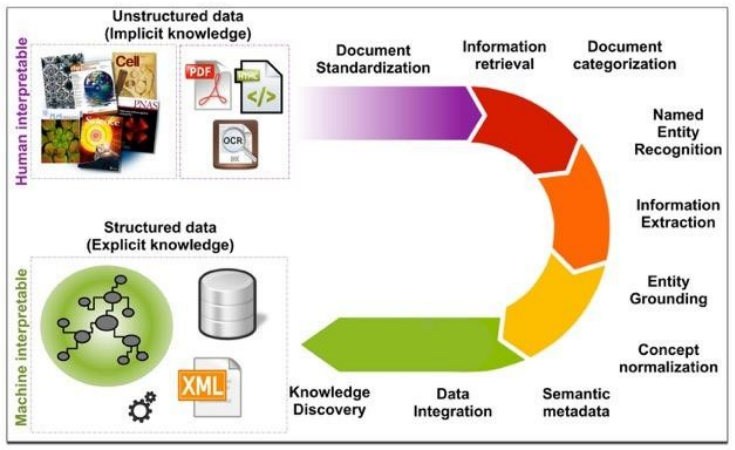
\includegraphics[width = 0.6\textwidth]{figs/biocuration.png}
\end{figure}

La biocuración es el proceso de recogida, verificación, organización y mantenimiento de datos biológicos para asegurar su calidad, coherencia y utilidad. En el contexto de la bioinformática, la biocuración implica seleccionar información relevante, estandarizarla y anotarla correctamente en bases de datos especializadas, facilitando así su análisis y reutilización en investigaciones científicas. El objetivo principal es transformar datos brutos en recursos confiables y estructurados que permitan realizar estudios precisos y reproducibles.

\begin{figure}[h]
\centering
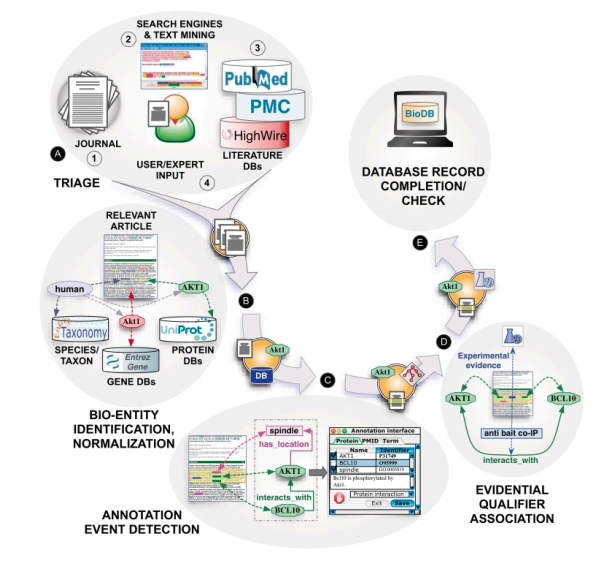
\includegraphics[width = 0.6\textwidth]{figs/biocuration2.png}
\end{figure}

Pese a la ayuda de la IA, la biocuración sigue siendo un proceso manual. Sus pasos son:
\begin{itemize}
\item Triaje: selección de artículos relevantes. El NLP clasifica el texto, detecta las entidades y tiene un aprendizaje no supervisado.
\item Normalización e identificación de bioentidades: hay varios nombres para una  misma patología, síntoma, causa, etc, por lo que se deben marcar como iguales. Por ejemplo: enfermedades vasculares hipertensivas, hipertensión e hipertensión arterial hacen alusión a lo mismo, pero con palabras distintas.
\item Anotación de eventos detectados: interacciones proteína-proteína, producción génica en cuanto a localización celular, etc, extracción de relaciones en general.
\item Asociación de calificadores probatorios
\item Comprobación y completar las entradas de la base de datos
\end{itemize}

Extraer relaciones entre entidades es una de las tareas más difíciles en
bioNLP. Es difícil porque, por un lado, es complicado extraer información significativa de la muestra para construir un modelo automático y, por otro lado, los modelos heurísticos no pueden abarcar todo el espectro de casos.

\subsection{Ontologías}
Más de 1500 bases de datos biológicas activas con datos y términos de diferentes campos y más de 200 vocabularios diferentes incluidos en recursos como UMLS: ontologías genéticas, secuencias genéticas, estructura proteica, terminología médica, taxonomías de especies, etc.

El UMLS (Unified Medical Language System) integra y distribuye terminología clave, normas de clasificación y
codificación, y recursos asociados para promover la creación de sistemas y servicios de información biomédica más eficaces e interoperables, incluidos los registros médicos electrónicos.

Originalmente integró 2 millones de nombres para unos 900 000 conceptos de más de 60 familias de vocabularios biomédicos, así como 12 millones de relaciones entre estos conceptos.
\begin{itemize}
\item Vinculación de términos con diccionarios estándar.
\item Exploración de ontologías de términos.
\item Búsqueda de relaciones entre términos.
\item Correspondencia entre uno y muchos de diferentes fuentes de bases de datos.
\end{itemize}

Los Medical Subject Headings (MeSH) son un vocabulario controlado y organizado jerárquicamente elaborado por la Biblioteca Nacional de Medicina. Se utiliza para indexar, catalogar y buscar información biomédica y relacionada con la salud.


%Exercise (5 min): Look at the repository PMC. Perform a query about the subject of the Jama article. Describe the structure of the query (righthadside window). Poner también la ontología MeSH